\documentclass[
	12pt,				% tamanho da fonte
	openany,			% capítulos começam em pág ímpar (insere página vazia caso preciso)
	oneside, 			% oneside - twoside
	a4paper,			% tamanho do papel.
	chapter=TITLE,		% títulos de capítulos convertidos em letras maiúsculas
	section=TITLE,		% títulos de seções convertidos em letras maiúsculas
	sumario=tradicional,	
	%subsection=TITLE,	% títulos de subseções convertidos em letras maiúsculas
	%subsubsection=TITLE,% títulos de subsubseções convertidos em letras maiúsculas
	english,			% idioma adicional para hifenização
	brazil,				% o último idioma é o principal do documento
	]{abntex2}

% ---------------------------------------------------------------------------
% Inclui os comandos do projeto
% ---------------------------------------------------------------------------
\input{tex/commands}

% ---------------------------------------------------------------------------
% IDENTIFICAÇÃO
% ---------------------------------------------------------------------------
\titulo{Desenvolvimento dirigido por comportamento aplicado em um sistema simulado de travamento de portas veicular}
\autor{Robson Luan do Nascimento de Sousa}
\local{Santa Inês - MA}
\orientador{Prof. Emanuel Cleyton Macedo Lemos, Msc.}
\coorientador{Prof. Aristoteles de Almeida Lacerda Neto, Dr.}
%\coorientador{M. Sc. Osvaldo Campelo de Mello Vasconselos}
\instituicao{
Instituto Federal do Maranhão
	\par
CURSO DE GRADUAÇÃO EM ENGENHARIA DE COMPUTAÇÃO}
\tipotrabalho{Trabalho de Conclusão de Curso}
\preambulo{Trabalho apresentado ao Instituto Federal do Maranhão, Campus Santa Inês, como requisito da obtenção do título de Bacharel em Engenharia de Computação.}


% -----------------------------------------------------------------------------
% CONFIGURACAO DO SUMARIO - by @Gabrielr2508
% Precisa estar aqui, por isso não foi para o commands.tex, não descobrimos o motivo, %caso saiba, por favor, faça um pull request! :D
% -----------------------------------------------------------------------------
% Secao primaria (Chapter) Caixa alta, Negrito, tamanho 12
\makeatletter
\renewcommand*{\l@chapter}[2]{%
  \l@chapapp{\uppercase{#1}}{#2}{\cftchaptername}}
\makeatother
% Secao secundaria (Section) Caixa baixa, Negrito, tamanho 12
\renewcommand{\cftsectionfont}{\uppercase} %ponha \rmfamily se quiser serifadas...

% Secao terciaria (Subsection) Caixa baixa, negrito, tamanho 12
\renewcommand{\cftsubsectionfont}{\bfseries}

% Secao quaternaria (Subsubsection) Caixa baixa, tamanho 12
\renewcommand{\cftsubsubsectionfont}{\normalfont}

% Seção quinaria (subsubsubsection) Caixa baixa, sem negrito, tamanho 12
\renewcommand{\cftparagraphfont}{\normalfont\itshape}

% Para possibilitar o uso de codigo
%\usepackage{minted}

\usepackage{listings}
\usepackage{xcolor} % Para customizar cores

\lstset{
  language=Python,        % ou C, C++, Java, etc.
  basicstyle=\ttfamily\footnotesize,
  numbers=left,
  numberstyle=\tiny,
  stepnumber=1,
  numbersep=5pt,
  backgroundcolor=\color{gray!10},
  frame=single,
  breaklines=true,
  captionpos=b,
  tabsize=2
}

% -----------------------------------------------------------------------------
% Início do TCC 
% -----------------------------------------------------------------------------
\begin{document}

	\frenchspacing % Retira espaço extra obsoleto entre as frases.
	
	\pretextual
		%--------------------------------------------------------------------------------
% Constrói a capa com base na seção de identificação do main.tex
%--------------------------------------------------------------------------------
\begin{capa}
    \setlength{\belowcaptionskip}{0pt}
    \setlength{\abovecaptionskip}{0pt}
    \setlength{\intextsep}{-18pt}
        \begin{figure}[h]
    		\begin{center}
    		    
\includegraphics[scale=.5]{img/ifma_novo.jpg}
    		\end{center}
    	\end{figure}

        %\includegraphics[scale=0.6]{img/univasf.jpg}
        \center
    	{\ABNTEXchapterfont\large\imprimirinstituicao}

    	\vspace*{2cm}
    	    {\imprimirautor}
    	\vspace*{2cm}
        \begin{center}
    		\ABNTEXchapterfont\bfseries\large\imprimirtitulo
        \end{center}
    	\vfill

    	\ABNTEXchapterfont\bfseries\large\imprimirlocal\\
    	\the\year

    	\vspace*{1cm}
\end{capa}
%--------------------------------------------------------------------------------
% Constrói a folha de rosto com base na seção de identificação do main.tex
%--------------------------------------------------------------------------------
\begin{folhaderosto}
    \center
    	{\ABNTEXchapterfont\large\imprimirinstituicao}

		\vspace*{2cm}
    	    {\imprimirautor}
    	\vspace*{2cm}
		\vspace*{\fill}

		{\ABNTEXchapterfont\bfseries\large\imprimirtitulo}
		\vspace*{\fill}

		{\hspace{.45\textwidth}
		\begin{minipage}{.5\textwidth}
			\SingleSpacing
			\imprimirpreambulo \\ \\

			{\imprimirorientadorRotulo~\imprimirorientador\par}
			{\imprimircoorientadorRotulo~\imprimircoorientador\par}

		\end{minipage}%
		\vspace*{\fill}}%
		\vspace*{\fill}
			\ABNTEXchapterfont\bfseries\large\imprimirlocal\\
			\the\year
		\vspace*{1cm}
\end{folhaderosto}

%--------------------------------------------------------------------------------
% Constrói a ficha catalográfia com base na seção de identificação do main.tex
% Está comentado porque no final das contas a biblioteca do seu campus que gera a
% numeração, você pode adicionar os numeros aqui, ou anexar o pdf gerado por eles
% ao documento.
%--------------------------------------------------------------------------------
%\begin{fichacatalografica}
%	\vspace*{\fill}					% Posição vertical
%	\hrule							% Linha horizontal
%	\begin{center}					% Minipage Centralizado
%	\begin{minipage}[c]{12.5cm}		% Largura
%
%	\imprimirautor
%
%	\hspace{0.5cm} \imprimirtitulo  / \imprimirautor. --
%	\imprimirlocal, \the\year-
%
%	\hspace{0.5cm} xx p. : il. (algumas color.) ; 30 cm.\\
%
%	\hspace{0.5cm} \imprimirorientadorRotulo~\imprimirorientador\\
%
%	\hspace{0.5cm}
%	\parbox[t]{\textwidth}{\imprimirtipotrabalho~--~\imprimirinstituicao,
%	\the\year.}\\
%
%	\hspace{0.5cm}
%		1. Palavra-chave1.
%		2. Palavra-chave2.
%		I. Orientador.
%		II. Universidade xxx.
%		III. Faculdade de xxx.
%		IV. Título\\
%
%	\hspace{8.75cm} CDU 02:141:005.7\\
%
%	\end{minipage}
%	\end{center}
%	\hrule
%\end{fichacatalografica}

%--------------------------------------------------------------------------------
% Anexando a ficha catalogáfica e a folha de aprovação
%--------------------------------------------------------------------------------
\includepdf[pages=-]{anexos/ficha.pdf}

\includepdf[pages=-]{anexos/aprovacao.pdf}

\setlength{\ABNTEXsignwidth}{12cm}

%--------------------------------------------------------------------------------
% Está comentado pelo mesmo motivo da ficha catalográfica
%--------------------------------------------------------------------------------
%\begin{folhadeaprovacao}
%	\begin{center}
%	    {\ABNTEXchapterfont\bfseries\large\imprimirinstituicao}
%	    \vspace*{\fill}
%
%	    {\ABNTEXchapterfont\bfseries\large FOLHA DE APROVAÇÃO}
%	    \vspace*{\fill}
%
%	    {\ABNTEXchapterfont\bfseries\large\imprimirautor}
%
%	    \vspace*{\fill}\vspace*{\fill}
%	    {\ABNTEXchapterfont\bfseries\large\imprimirtitulo}
%	    \vspace*{\fill}
%
%	    {\hspace{.45\textwidth}
%		\begin{minipage}{.5\textwidth}
%			\SingleSpacing
%			\ABNTEXchapterfont\imprimirpreambulo \\ \\
%
%			{\ABNTEXchapterfont\imprimirorientadorRotulo~\imprimirorientador\par}
%			{\ABNTEXchapterfont\imprimircoorientadorRotulo~\imprimircoorientador\par}
%
%		\end{minipage}%
%	    \vspace*{\fill}}
%	\end{center}
%
%	\vspace*{\fill}
%
%	\begin{center}
%			 \ABNTEXchapterfont\large Aprovado em: \_\_\_\_ de \_\_\_\_ de 2017
%	\end{center}

%	\vspace*{\fill}

%	\begin{center}
%			 \ABNTEXchapterfont\bfseries\large Banca Examinadora
%	\end{center}
%
%   \ABNTEXchapterfont\assinatura{Fábio Nelson de Sousa Pereira, Mestre, Universidade Federal do Vale do São Francisco}
%	\ABNTEXchapterfont\assinatura{Jorge Luis Cavalcanti Ramos, Doutor, Universidade Federal do vale do São Francisco}
%  \ABNTEXchapterfont\assinatura{Ricardo Argenton Ramos, Doutor, Universidade Federal do Vale do São Francisco}
%	 \vspace*{\fill}


%\end{folhadeaprovacao}

%--------------------------------------------------------------------------------
% Insere a epígrafe
%--------------------------------------------------------------------------------
\newpage
\vspace*{\fill}
\begin{flushright}
		\textit{Lorem Ipsum...}
\end{flushright}

%--------------------------------------------------------------------------------
% Seção de agradecimentos
%--------------------------------------------------------------------------------
\begin{agradecimentos}

\lipsum[2-4]

\end{agradecimentos}

%--------------------------------------------------------------------------------
% Insere a segunda epígrafe
%--------------------------------------------------------------------------------
\begin{epigrafe}
    \vspace*{\fill}
	\begin{flushright}
		Se pude enxergar a tão grande distância, foi subindo nos ombros de gigantes.\\
		 \vspace{\baselineskip}
		\textbf{Isaac Newton}\\
		\textbf{Carta à Robert Hooke, 1676}
	\end{flushright}
\end{epigrafe}



%--------------------------------------------------------------------------------
% Seção de resumos
%--------------------------------------------------------------------------------
% resumo em português
\setlength{\absparsep}{18pt} % ajusta o espaçamento dos parágrafos do resumo
\begin{resumo}

\lipsum[1-2]

 \textbf{Palavras-chave}: \textit{Palavra em inglês 1, Palavra em inglês 2, Palavra em inglês 3, Palavra em inglês 4}, Palavra 5.

\end{resumo}

%---------------------------------------------------------------------------------
% resumo em inglês
\begin{resumo}[Abstract]
\begin{otherlanguage*}{english}

\lipsum[3-4]

	\vspace{\onelineskip}

	\noindent
	\textbf{Key-words}: \textit{Palavra em inglês 1, Palavra em inglês 2, Palavra em inglês 3, Palavra em inglês 4, Palavra em inglês 4}.

\end{otherlanguage*}
\end{resumo}


%---------------------------------------------------------------------------------
% Insere lista de ilustrações
%---------------------------------------------------------------------------------
\begin{KeepFromToc} % Este comando evita que todas as seções dentro dele de apareçam no sumário
\pdfbookmark[0]{\listfigurename}{lof}
\listoffigures
%\addcontentsline{toc}{chapter}{Lista de Figuras}
\cleardoublepage


%---------------------------------------------------------------------------------
% Insere lista de tabelas
%---------------------------------------------------------------------------------
\pdfbookmark[0]{\listtablename}{lot}
\listoftables
\cleardoublepage

%---------------------------------------------------------------------------------
% Insere lista de quadros
%---------------------------------------------------------------------------------
\pdfbookmark[0]{\listofquadrosname}{loq}
\listofquadros*
\cleardoublepage

%---------------------------------------------------------------------------------
% Ajusta lista de código - alterar de figures para códigos - by @Gabrielr2508
%---------------------------------------------------------------------------------
\makeatletter
\let\l@listing\l@figure
\def\newfloat@listoflisting@hook{\let\figurename\listingname}
\makeatother

%---------------------------------------------------------------------------------
% Insere lista de códigos - by @leolleocomp
%---------------------------------------------------------------------------------
\listoflistings

\end{KeepFromToc}

%---------------------------------------------------------------------------------
% Insere lista de abreviaturas e siglas
%---------------------------------------------------------------------------------
\begin{siglas}
	\item[LI]       Lorem Ipsum
    \item[LII]		Lorem Ipsum Ipsum

\end{siglas}

%---------------------------------------------------------------------------------
% Insere o sumario
%---------------------------------------------------------------------------------
\pdfbookmark[0]{\contentsname}{toc}
\tableofcontents*
\cleardoublepage




	\textual
		\pagestyle{simple}
		%--------------------------------------------------------------------------------------
% Este arquivo contém a sua introdução, objetivos e organização do trabalho
%--------------------------------------------------------------------------------------
\chapter{Introdução}

A indústria automotiva tem experimentado um crescimento constante, acompanhado por um aumento significativo na modernização dos veículos e pela intensa competição entre 
montadoras para entregar produtos cada vez mais robustos e de alta qualidade. Esse cenário traz consigo um aumento na complexidade do desenvolvimento, demandando soluções 
mais eficientes e seguras para sistemas cada vez mais sofisticados e que sejam capazes de atender às necessidades específicas de cada cliente.

A modernização do setor automotivo tem conduzido ao próximo grande avanço: os veículos definidos por software (\textit{Software-Defined Vehicles}) 
\cite{softwareVehicles2025}. Essa abordagem possibilita a customização contínua e a evolução do produto mesmo após a aquisição, permitindo a entrega de novas 
funcionalidades ao veículo por meio de atualizações de software feitas remotamente \textit{Over-the-Air (OTA)}, suportadas pelo hardware já embarcado.

Diante desse contexto, a Engenharia Automotiva enfrenta o desafio de projetar e desenvolver produtos com um nível altíssimo de qualidade, ao mesmo tempo em que busca reduzir 
erros e retrabalho. A aplicação de metodologias ágeis, como o \textit{Behavior Driven Development (BDD)} \cite{north2006bdd}, oferece uma abordagem promissora, pois foca na 
definição do comportamento esperado do sistema a partir da perspectiva do usuário. Essa abordagem permite uma colaboração mais efetiva entre os membros de uma equipe ágil 
\cite{atlassianAgileTeams}, facilita a descoberta de funcionalidades e possibilita que o desenvolvimento seja guiado por testes de aceitação automatizados, promovendo 
entregas de valor de forma mais rápida e com maior confiabilidade.

\section{\textbf{Justificativa}}

O problema central deste trabalho é: ``como é possível aplicar o processo de BDD para facilitar a definição do sistema e guiar seu desenvolvimento no contexto da 
Engenharia de Sistemas Automotivos?''. A solução proposta consiste na adaptação do processo, integrando as técnicas já consolidadas do BDD com metodologias 
amplamente utilizadas na indústria automotiva, de forma a lidar com as complexidades inerentes ao desenvolvimento de sistemas veiculares.

Este trabalho insere-se no contexto atual da indústria automotiva, adotando o sistema de travamento de portas como prova de conceito para a geração do produto. 
Durante seu desenvolvimento, serão consideradas como referência implementações reais de sistemas já presentes em veículos, como os da Volkswagen \cite{vwLocking} 
e da Bosch \cite{bosch2022handbook,reif2017locking}. Nesse sentido, a adaptação do processo de BDD será aplicada ao desenvolvimento de um produto compatível com 
as especificações industriais, ao mesmo tempo em que busca minimizar as complexidades enfrentadas em sua execução.

O BDD incorpora diversas premissas que surgem das lições aprendidas na aplicação de outras metodologias ágeis, definindo o desenvolvimento do produto a partir do 
comportamento que gera valor ao usuário. Além disso, ele busca promover a colaboração entre as diferentes etapas do desenvolvimento, garantindo que toda a equipe 
compreenda o produto e consiga assumir a perspectiva do usuário.

Por outro lado, a Engenharia Automotiva apresenta uma complexidade significativa, o que torna desafiadora a entrega de produtos de alta qualidade. A definição de 
um sistema veicular envolve muito mais do que software ou eletrônica, sendo necessário integrar componentes mecânicos, considerar falhas 
potenciais, garantir a rastreabilidade de requisitos e contemplar casos de uso extremos.

O principal desafio deste trabalho consiste em identificar técnicas capazes de capturar as complexidades envolvidas no desenvolvimento de sistemas automotivos 
e adaptá-las às premissas do BDD. Em casos como o do sistema de travamento de portas, isso é traduzido na necessidade de atender a funcionalidades 
essenciais, como (GSMH, 2022):

\begin{itemize}
    \item Permitir o acesso ao interior do veículo para todas as pessoas autorizadas;
    \item Gerenciar a abertura das portas a partir das maçanetas internas e externas;
    \item Proteger os ocupantes da abertura indevida das portas;
    \item Proteger o veículo contra furtos enquanto ele está estacionado.
\end{itemize}

Uma das principais complexidades desse tipo de sistema está na definição do mecanismo empregado no travamento das portas. Conforme descrito por 
\citeonline{reif2017locking}, podem ser utilizadas travas mecânicas ou eletrônicas, cada um com conjuntos específicos de componentes e lógicas de 
software distintas que influenciam diretamente o desenvolvimento. Esse desafio é recorrente na indústria automotiva, na qual diversos sistemas dependem 
de decisões técnicas de hardware ou soluções mecânicas para viabilizar o início do processo de design.

Neste trabalho, será apresentada uma metodologia que demonstra como a aplicação do Desenvolvimento Orientado a Comportamento (BDD) possibilita projetar o 
sistema de forma independente dos detalhes técnicos, facilitando tanto o desenvolvimento das funcionalidades quanto a execução dos testes. Isso ocorre 
porque a abordagem do BDD prioriza a perspectiva do usuário e a especificação do comportamento esperado do sistema, os quais não estão diretamente vinculados 
à implementação.

\section{\textbf{Objetivos}}

\subsection{Objetivo Geral}
%Para responder à problemática levantada, o presente estudo tem como objetivo geral 
Aplicar o levantamento e definição de funcionalidades na análise de um sistema de travamento de portas veicular, seguido do desenvolvimento guiado por testes de 
aceitação automatizados, demonstrando como essas práticas podem contribuir para o desenvolvimento de software automotivo de forma mais organizada e eficiente.

\subsection{Objetivos Específicos}
\begin{itemize}
    \item Realizar o levantamento e definição de funcionalidades considerando possíveis limitações decorrentes da dependência de hardware e de sistemas mecânicos;
	\item Analisar as complexidades dos sistemas automotivos de maneira compatível com o processo de BDD;
    \item Empregar técnicas de desenvolvimento como padrão de escrita de software AUTOSAR \cite{autosarClassic} e Design Orientado por Modelos (\textit{Model-Based Desgin - MBD}) \cite{mathworksMBD2024}, que são amplamente utilizadas na indústria automotiva;
    \item Definir um escopo de desenvolvimento que possibilite a realização do design do sistema forma clara e compreensível;
    \item Empregar testes de aceitação automatizados para guiar o desenvolvimento do sistema, consistente com o design definido;
    \item Realizar a implementação do sistema de maneira iterativa, possiblitando à descoberta de melhorias surgidas durante a aplicação do processo;
    \item Aplicar a metodologia desenvolvida na produção de um sistema de travamento de portas veicular simulado.
\end{itemize}

% \section{Metodologia}

% A metodologia utilizada neste estudo baseia-se na revisão da bibliografia disponível, com o objetivo de esclarecer o processo de BDD e investigar como ele pode 
% ser adaptado para incorporar práticas consolidadas na Engenharia Automotiva. Para tanto, serão aplicadas técnicas como o mapeamento de exemplos 
% \cite{Lawrence2019cucumber, cucumberExampleMapping}
% , voltado ao levantamento e definição de funcionalidades, e testes de aceitação automatizados 
% \cite{studyBDD}
% , que servirão para guiar o desenvolvimento do sistema.

% A implementação do sistema simulado também fará uso de técnicas típicas da Engenharia Automotiva, incluindo o Model Based Design
% \cite{Vincentelli2001, mathworksMBD2024} e a geração automática de código segundo o padrão de software AUTOSAR 
% \cite{autosarClassic}. Conceitos adicionais do domínio automotivo serão considerados para 
% assegurar a adequada abstração nas diferentes etapas do desenvolvimento.

% Espera-se que os resultados obtidos evidenciam os benefícios da integração do BDD no contexto automotivo, destacando sua contribuição para a qualidade e 
% confiabilidade do sistema. A validação será realizada por meio da execução dos testes de aceitação e da análise do uso do sistema final sob a perspectiva do usuário.

\section{\textbf{Organização do trabalho}}
No Capítulo \ref{ch:te}, serão apresentados os conceitos que compõem a fundamentação teórica deste trabalho, abrangendo:

\begin{itemize}
    \item \textbf{O processo de BDD} - histórico do desenvolvimento do processo e seus pilares fundamentais do processo;
    \item \textbf{Mapeamento de exemplos} - metodologia aplicada para realizar a análise do sistema e definição de funcionalidades;
    \item \textbf{A linguagem \textit{Gherkin}} - linguagem usada para a escrita de cenários, que atuam como definição de comportamentos e como testes de aceitação;
    \item \textbf{Design orientado por modelo} - metodologia adotada para a implementação do sistema;
    \item \textbf{Sistemas de travamento de porta veiculares} - definição e caracterização dos sistemas de segurança voltados ao travamento de portas em veículos. 
\end{itemize}

Em seguida, no Capítulo \ref{ch:MM}, será apresentada a metodologia adotada, descrevendo o procedimento de desenvolvimento do produto, estruturado em seis etapas. 
Serão também detalhadas as ferramentas utilizadas neste trabalho, bem como os critérios de avaliação, definidos a partir da execução dos testes de aceitação de 
cada funcionalidade do sistema.

No Capítulo \ref{ch:IM}, a implementação é conduzida por meio da execução das quatro primeiras etapas do processo. Essa fase tem início com a definição das histórias 
de usuário — que representam as funcionalidades do sistema — conforme descrito na Seção \ref{sbs:etapa1}. A histórias orientam todas as etapas subsequentes, desde a 
elaboração dos testes de aceitação até a modelagem do sistema.

Para cada história de usuário, o mapeamento de exemplos, descrito na Seção \ref{sbs:etapa2}, será empregado para orientar a definição dos detalhes relacionados 
ao comportamento esperado. Em seguida, na Seção \ref{sbs:etapa3}, o sistema será modelado como uma abstração que explicita as interações com o usuário, ao mesmo 
tempo em que oculta os aspectos técnicos de sua implementação. A partir das histórias de usuário e do modelo do sistema, será elaborada, na Seção \ref{sbs:etapa4}, 
uma série de cenários que representam tanto a especificação do comportamento esperado quanto os testes de aceitação correspondentes.  

No capítulo \ref{ch:RD}, será feita a execução dos testes de validação que foram criados ao fim do capítulo \ref{ch:IM}. Esse processo é feito para garantir 
que a modelagem do sistema é guiada a partir dos cenários desenvolvidos e satisfaz o comportamento definido como uma forma de resolver erros capturados na execução 
dos testes. 

No Capítulo \ref{ch:RD}, serão executados os testes de validação definidos pelos cenários das histórias de usuário. Esse processo assegura que a modelagem do sistema 
seja orientada pela execução dos testes e que o comportamento especificado seja atendido. Ela também possibilita a identificação e a correção de falhas detectadas 
durante a execução dos testes.

A aprovação das histórias de usuário será realizada a partir da verificação de que:

\begin{itemize}
    \item Os testes foram executados e confirmaram a aprovação de todos os cenários relacionados à história;
    \item A execução dos cenários é repetida ao longo do desenvolvimento das demais histórias, de modo a assegurar que o comportamento previamente validado não seja comprometido.
\end{itemize}

Por fim, no Capítulo \ref{ch:CC}, será apresentada uma síntese dos principais aspectos observados durante a aplicação da metodologia proposta. Adicionalmente, serão 
discutidas algumas limitações do escopo deste trabalho, acompanhadas de sugestões de continuidade para o desenvolvimento futuro que culminam na geração do produto físico.

		%--------------------------------------------------------------------------------------
% Este arquivo contém a sua funtamentação teórica
%--------------------------------------------------------------------------------------
\chapter{Fundamentação teórica}

\section{Seção de exemplo 1 - Como fazer citações}

Existem vários tipos de citações...


\section{Seção de exemplo 2 - Como inserir figuras}

Neste trabalho iremos exemplificar duas formas de se inserir figuras no Latex. O primeiro método insere, no documento, uma figura simples por meio do comando:

\textbackslash imagem\{ Escala \}\{ Arquivo sem extensão \}\{ Descrição \}\{ Fonte \}

\textbf{Obs.:} A fonte pode ser uma citação do tipo  \textbackslash citeonline\{\}.

% A figura \ref{img:placeholder} é um exemplo deste método.

% %--------------------------------------------------------------------------------------
% % Esse é um exemplo de figura simples
% %--------------------------------------------------------------------------------------
% \imagem{0.15}{placeholder}{Uma figura simples}{O autor}

% A figura \ref{img:figura1} é um exemplo do outro tipo de figura abordada aqui, chamada de figura composta. Esta figura é composta de outras subfiguras.
% %--------------------------------------------------------------------------------------
% % Esse é um exemplo de figura composta de outras subfiguras
% %--------------------------------------------------------------------------------------
% \begin{figure}[!htb]
% \centering
%     \caption{\label{img:figura1} Exemplo de figura composta}
%     \subcaptionbox{\label{img:subfigura1} Subfigura 1}{\includegraphics[scale=.1]{img/placeholder}}\qquad
%     \subcaptionbox{\label{img:subfigura2} Subfigura 2}{\includegraphics[scale=.1]{img/placeholder}}
%     \vspace{1.5em}
%     \legend{\textbf{Fonte:} \citeonline{SUA-REFERENCIA}}
% \label{fig:dag}
% \end{figure}

%\begin{figure}[!htb]
%\centering
%    \caption{\label{img:telas} Telas da aplicação cliente}
%    \subcaptionbox{\label{img:inicial} Abertura}{\includegraphics[scale=.12]{img/APP/inicial}}\qquad
%    \subcaptionbox{\label{img:login} \textit{Login}}{\includegraphics[scale=.12]{img/APP/login}}\qquad
%    \subcaptionbox{\label{img:cadastro} Cadastro}{\includegraphics[scale=.12]{img/APP/cadastro}}\qquad
%    \subcaptionbox{\label{img:hist-rel}Sobre}{\includegraphics[scale=.12]{img/APP/sobre}}\\
%    \vspace{1.5em}
%    \subcaptionbox{\label{img:dados_atuais}Dados atuais}{\includegraphics[scale=.15]{img/APP/atual}}\qquad
%    \subcaptionbox{\label{img:hist-time}Seleção de período}{\includegraphics[scale=.15]{img/APP/periodo}}\qquad
%    \subcaptionbox{\label{img:hist-rel}Exibir histórico}{\includegraphics[scale=.15]{img/APP/historico}}\\
%    \vspace{2.5em}
%    \legend{\textbf{Fonte:} O Autor}
%\label{fig:dag}
%\end{figure}

\begin{figure}[ht]
\centering
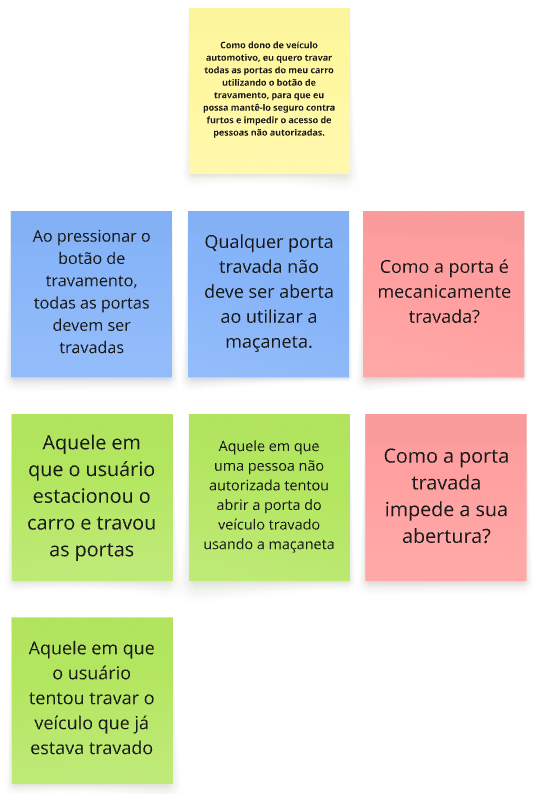
\includegraphics[height=12cm]{figuras/user_story_1.png}
\caption{História de Usuário 1: Travamento de todas as portas}
%\label{fig:casos-uso}
\end{figure}

\begin{figure}[ht]
\centering
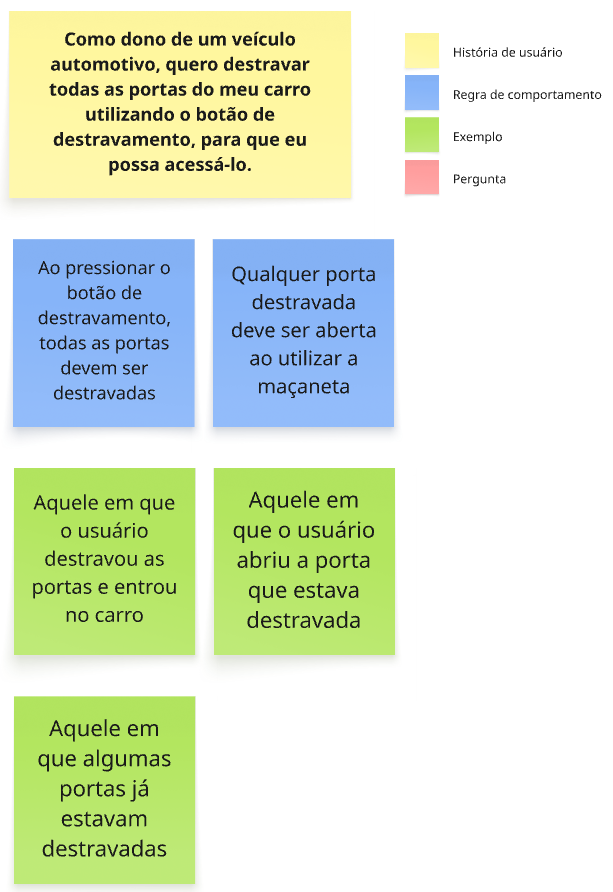
\includegraphics[height=12cm]{figuras/user_story_2.png}
\caption{História de Usuário 2: Destravamento de todas as portas}
%\label{fig:casos-uso}
\end{figure}

\begin{figure}[ht]
\centering
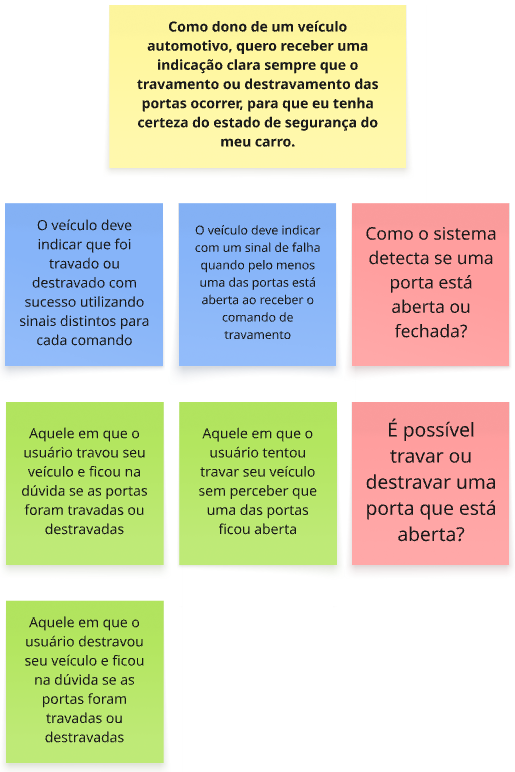
\includegraphics[height=12cm]{figuras/user_story_3.png}
\caption{História de Usuário 3: Feedback de travamento}
%\label{fig:casos-uso}
\end{figure}

\begin{figure}[ht]
\centering
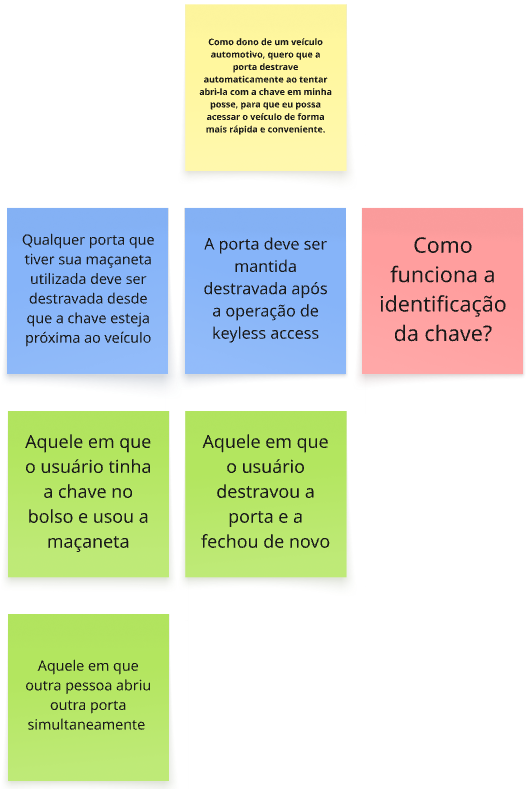
\includegraphics[height=12cm]{figuras/user_story_4.png}
\caption{História de Usuário 4: Keyless Access}
%\label{fig:casos-uso}
\end{figure}

\begin{figure}[ht]
\centering
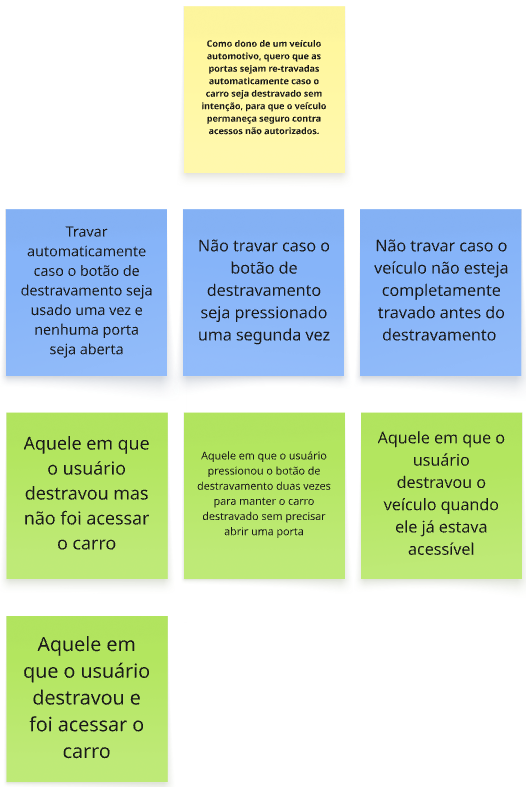
\includegraphics[height=12cm]{figuras/user_story_5.png}
\caption{História de Usuário 5: Travamento automático}
%\label{fig:casos-uso}
\end{figure}

Para referenciar uma figura deve ser usada comando \textbackslash ref\{img:<label ou nome do arquivo>\}, como exemplo, estamos referenciando a figura \ref{img:placeholder}. Isso vale tanto para figuras simples quanto para as compostas, como por exemplo as figuras \ref{img:subfigura1} e \ref{img:subfigura2}. Ao inserir uma figura, ela é automaticamente identificada e incluída no elemento pré-textual da lista de figuras.




\section{Seção de exemplo 3 - Sobre tabelas}

As tabelas em Latex são deveras capciosas, por isso não serão abordadas em sua completude neste documento.

Há um site que possui uma ferramenta interessante para ser utilizada na construção tabelas em Latex.

\centerline{\href{https://www.tablesgenerator.com/}{ O Tables Generator } <-- Isto é um \textit{link} :D}

Contudo, busquem entendimento sobre o assunto, pois tabelas são elementos textuais importantes e enriquecem muito o texto, quando bem construídas.

A tabela \ref{tab:crossplatform} é um exemplo de como uma tabela pode ser construída, assim como a tabela do anexo \ref{anex:anexo1}.

\begin{table}[!htb]
	\centering
	\caption{\label{tab:crossplatform} Tipos de aplicações e abordagens preferenciais.}
	\begin{adjustbox}{max width=\textwidth}
		\begin{tabular}{@{} p{5cm} |c|c|c| @{}}
		\toprule
		\textbf{Código da Aplicação} & \textbf{Web} & \textbf{Híbrida} & \textbf{Interpretada / Compilação Cruzada} \\ \hline

		\textbf{Aplicações baseadas em dados providos por um servidor} &
			3 & 2 & 1
		\\ \hline

		\textbf{Aplicações independentes} & 1 & 2 & 3\\ \hline

		\textbf{Aplicações baseadas em sensores e processamento de dados no dispositivo} & 1 & 2 & 3\\ \hline

		\textbf{Aplicações baseadas em sensores e processamento de dados no servidor} & 1 & 3 & 2\\ \hline

		\textbf{Aplicações Cliente-Servidor} & 1 & 3 & 2 \\ \bottomrule
	\end{tabular}
	\end{adjustbox}
	\legend{\textbf{Fonte:} \citeonline{raj2012study} (Traduzido)}
\end{table}

Também é possível criar quadros, que são ligeiramente diferente de tabelas. Acompanhe o exemplo no Quadro \ref{qua:confusionmatrix}

\begin{quadro}
	\centering
	\caption{\label{qua:confusionmatrix}Exemplo de matriz de confusão}
	\begin{tabular}{ll|c|c|}
		\cline{3-4}
		\multicolumn{1}{c}{\textbf{}} & \multicolumn{1}{c|}{\textbf{}} & \multicolumn{2}{l|}{\textbf{Classe prevista}} \\ \cline{3-4}
		 & \multicolumn{1}{c|}{\textbf{}} & Classe = 1 & Classe = 0 \\ \hline
		\multicolumn{1}{|l|}{\multirow{2}{*}{\textbf{Classe real}}} & Classe = 1 & $f_{11}$ & $f_{10}$ \\ \cline{2-4}
		\multicolumn{1}{|l|}{} & Classe = 0 & $f_{01}$ & $f_{00}$ \\ \hline
	\end{tabular}
	\Ididthis
\end{quadro}


\begin{quadro}
	\caption{\label{qua:cron}Cronograma}
	\center
	\begin{tabular}{|c|c|c|c|c|c|}
	\hline
	\multicolumn{1}{|l|}{Atividade} & \multicolumn{1}{l|}{Set/19} & \multicolumn{1}{l|}{Out/19} & \multicolumn{1}{l|}{Nov/19} & \multicolumn{1}{l|}{Dez/19} & \multicolumn{1}{l|}{Jan/20} \\ \hline
	1                               & x                           &                             &                             &                             &                             \\ \hline
	2                               &                             & x                           &                             &                             &                             \\ \hline
	3                               &                             & x                           &                             &                             &                             \\ \hline
	4                               &                             &                             & x                           & x                           &                             \\ \hline
	5                               &                             & x                           & x                           & x                           &                             \\ \hline
	6                               &                             &                             &                             &                             & x                           \\ \hline
	
	\end{tabular}
	\legend{\textbf{Fonte:} Elaborado pela autora (2019)}
	\end{quadro}

\section{Subseção de exemplo 4 - Seções}

		%%--------------------------------------------------------------------------------------
% Este arquivo contém a sua metodologia
%--------------------------------------------------------------------------------------
\chapter{Metodologia} \label{ch:MM} %Uma label é como você referencia uma seção no texto com a tag \ref{}
Neste capítulo, será apresentada a metodologia aplicada para o desenvolvimento deste produto do Trabalho de Conclusão de Curso (TCC), que possui natureza técnica 
e tem como objetivo o desenvolvimento de um sistema integrado de travamento de portas veicular, quais as ferramentas utilizadas e como o Desenvolvimento Baseado 
em Comportamento (BDD) foi empregado.

\section{\textbf{Tipo de Pesquisa}} 
Esta é uma pesquisa aplicada, tendo em vista à solução de problemas presentes em metodologias de desenvolvimento de produto tradicionais como rastreabilidade 
de requisitos e aplicação de testes manuais. Também será aplicada uma abordagem mista, que demonstra quantitativamente a cobertura dos testes desenvolvidos em 
Modelo em Loop (MIL) e qualitativamente na experiência de usuário no modelo final.

\section{\textbf{Procedimentos Metodológicos}}
Este produto teve seu desenvolvimento em etapas com base na metodologia do processo de BDD como demonstrado em \citeonline{studyBDD}, com uma série de adaptações específicas 
para o contexto da Engenharia Automotiva. As etapas de desenvolvimento a seguir serão aplicadas:
\begin{enumerate}
    \item Descrição das histórias de usuário: Capturar as histórias definidas em forma de requisitos funcionais com linguagem natural e que capture o valor 
    gerado pela perspectiva do usuário;
    \item Mapeamento de exemplos: Definição de exemplos concretos tomados da perspectiva do usuário final;
    \item Desenho do diagrama de caixa preta: Desenho do diagrama do sistema que demonstra suas interfaces de entrada e saída, sem demonstrar detalhes de suas interações;
    \item Desenvolvimento dos cenários Gherkin: Escrita dos cenários aplicando o padrão cucumber e que aborde todas as regras definidas;
    \item Tradução dos cenários em testes: Desenvolvimento de funções dos passos dos cenários gherkin utilizando as interfaces do diagrama de caixa branca;
    \item Modelagem iterativa do sistema em simulink: Modelagem feita de forma iterativa aplicando os cenários como critério de aceitação a cada iteração;
    \item Análise qualitativa do produto final: Testes de uso do produto final e aprovação da experiência de usuário entregue.
\end{enumerate}

Neste projeto, algumas etapas serão repetidas, pois o desenvolvimento orientado por comportamento (BDD) é um processo incremental, baseado em iterações 
sucessivas que introduzem novas funcionalidades ao produto. Assim, as etapas 1 e 2 serão inicialmente executadas para cada história de usuário. Ao final 
desse ciclo, a etapa 3 será iniciada elaborando um diagrama de caixa preta que abrange todas as funcionalidades definidas até o momento.

\section{\textbf{Ferramentas Utilizadas}}
As ferramentas e tecnologias adotadas no desenvolvimento deste produto foram escolhidas com base na compatibilidade com o modelo proposto e na sua capacidade 
de integrar diferentes etapas do processo. A seguir, descreve-se cada uma delas:

\begin{itemize}
    \item \textbf{Cucumber (Gherkin)}: utilizado como padrão para a escrita de cenários comportamentais, permitindo a especificação dos requisitos no formato Given-When-Then, de forma legível por humanos e máquinas;
    \item \textbf{Miro}: empregado para a criação de diagramas não técnicos, bem como para auxiliar na discussão colaborativa de exemplos, fluxos e histórias de usuário;
    \item \textbf{Visual Studio Code}: ambiente de desenvolvimento (IDE) utilizado para escrever os cenários em Gherkin, desenvolver a tradução para testes executáveis e integrar o código gerado ao microcontrolador;
    \item \textbf{Python}: linguagem escolhida para implementar a lógica de tradução dos cenários Gherkin em testes executáveis, permitindo automatização e validação do comportamento esperado do sistema.
    \begin{itemize}
        \item \textbf{Behave}: biblioteca utilizada para interpretar e executar os cenários comportamentais no formato BDD, integrando as especificações Gherkin à lógica de teste.
        \item \textbf{Matlab Engine API for Python}: biblioteca usada para permitir a comunicação entre scripts Python e o ambiente Simulink, possibilitando a execução dos testes durante a simulação.
    \end{itemize}    
    \item \textbf{Simulink}: ferramenta adotada para a modelagem do sistema embarcado funcional, possibilitando simulações e geração automática de código C para o sistema-alvo.
    \item \textbf{Git/Github}: utilizado para o versionamento do projeto que inclui o modelo simulink do sistema, código embarcado gerado do modelo, arquivos feature dos cenários gherkin e códigos python dos testes executáveis.

\end{itemize}

\section{\textbf{Critérios de Avaliação}}
Para a verificação e validação do produto gerado, serão aplicados critérios quantitativos de análise, com base nos testes de aceitação de cada história de usuário. Este 
processo será realizado durante a etapa 6, correspondente à modelagem iterativa do sistema no Simulink.

A cada iteração, os testes de aceitação de uma história de usuário serão executados e, com base nos cenários não aprovados, serão identificadas falhas no comportamento 
do modelo. A partir dessas falhas, serão implementadas soluções para garantir a aprovação dos testes que podem envolver ajustes na lógica do modelo, 
alterações na escrita dos cenários Gherkin ou atualizações nas funções de definição de passos.

Após a aprovação dos testes de uma história, todos os cenários previamente aprovados serão reexecutados. Dessa forma, é possível verificar que modificações realizadas 
para atender a um cenário específico não impactaram os demais, garantindo a robustez do sistema.

Ao final do processo, todos os cenários de todas as histórias de usuário serão executados em conjunto, assegurando que o produto final atenda a todas as funcionalidades 
mapeadas e que 100\% dos testes de aceitação sejam aprovados.

%--------------------------------------------------------------------------------------
% Insere a seção de cronograma
% Está comentada porque só é necessária no TCC I
%--------------------------------------------------------------------------------------

%\section{Cronograma} \label{sec:crono}

%A tabela \ref{tab:cronograma} mostra o cronograma de atividades a serem executadas para o TCC II, com base no calendário de 201X.Y da UNIVASF.

%\newpage
%\begin{table}[!thb]
%	%\huge
%    \centering
%    \caption{\label{tab:cronograma} Cronograma das atividades previstas para o TCC II}
%%    \begin{adjustbox}{max width=\textwidth}
%    \begin{tabular}{p{6.5cm}|c|c|c|c|c|c}
%    \toprule
%    \textbf{Atividade}                      & Nov & Dez & Jan & Fev & Mar & Abr \\ \hline
%    Implementar o banco de dados              & X    & X     &       &        &          &          \\ \hline
%    Desenvolver a API HTTP RESTful                      &   X   & X     &       &        &          &          \\ \hline
%    Implementar o serviço de captura de dados        &      &      & X     &   X     &          &          \\ \hline
%    Desenvolver a aplicação \textit{Web/mobile} para exibição dos dados         &      &      & X     &   X     &     X     &          \\ \hline
 %   Teste do sistema            &      &       &       &        & X        &          %\\ \hline
 %   Escrita do TCC II                       &   X   & X     & X     & X      & X        & X        \\ \hline
%   Defesa do TCC II                        &      &       &       &        &          & X       \\
%    \bottomrule
 %   \end{tabular}
 %   \end{adjustbox}
%    \legend{\textbf{Fonte:} O autor.}
%\end{table}


		%\chapter{Resultados} \label{ch:RD}



% \section{Seção de exemplo 1 - Códigos} \label{sec:resex1}

% \subsection{Subseção de exemplo 1 - Inserindo trechos de códigos}
 
% O nosso querido Leonardo Cavalcante providenciou um comando que deixa nossos trechos de códigos bonitinhos e gera um elemento pré-textual de Lista de Códigos. 

% Os códigos são adicionados através do comando seguinte:

% \textbackslash sourcecode\{ Descrição \}\{Label\}\{Linguagem\}\{Arquivo com extensão\}

% Um exemplo pode ser visto no código \ref{cmd:cron} abaixo.

% %\sourcecode{Configuração do intervalo de execução no Script Agendador}{cron}{javascript}{cron.js}


% \section{Seção de exemplo 2 - Listas} \label{sec:resex2}

% \subsection{Subseção de exemplo 2 - Lista de itens} 

% Existem alguns tipos de listas no Latex, iremos exemplificar a lista sem numeração (seção \ref{subsubsec:itemize}), a lista enumerada (seção \ref{subsubsec:enumerate}) e a lista mista (seção \ref{subsubsec:mista}). As listas podem ser encadeadas de diversas maneiras,
% de acordo com a necessidade do autor.

% \subsubsection{Subsubseção de exemplo 1 - Lista sem numeração} \label{subsubsec:itemize}

% Este é um exemplo de lista sem numeração.

% \begin{itemize}
% 	\item \textbf{Cadastrar usuário}

% 		\begin{itemize}
%     		\item Atores
% 		    	\begin{itemize}
%     		    	\item Usuário
% 		    	\end{itemize}

% 	    	\item Fluxo de eventos primário
% 			    \begin{itemize}
% 	    		    \item o usuário deve se cadastrar informando seu nome, \textit{e-mail} e senha;
% 		        	\item a API armazena os dados do usuário;
% 		    	    \item o usuário é liberado para realizar o \textit{login}.
% 			    \end{itemize}

%     		\item Fluxo alternativo
% 			    \begin{itemize}
% 		    	   \item o usuário desiste de se cadastrar e cancela o caso de uso clicando no botão voltar.
% 	    		\end{itemize}

% 		\end{itemize}
	
% \end{itemize}

% \subsubsection{Subsubseção de exemplo 2 - Lista enumerada} \label{subsubsec:enumerate}

% Este é um exemplo de lista enumerada.

% \begin{enumerate}
% 	\item O Usuário deseja ver o histórico das variáveis climáticas, então através da interface de usuário escolhe o período ao qual o histórico se refere;
% 	\item A aplicação solicita à API através de uma requisição HTTP contendo o momento de início e o momento do fim do período em seus parâmetros;     			\item A API recebe a solicitação e se comunica com a base de dados, então requere as informações quem possuem a data de leitura no intervalo escolhido;
% 	\item A base de dados retorna os dados em formato Json para a API;
% 	\item A API responde à requisição retornando os dados, também em formato Json, para a aplicação cliente;
% 	\item A aplicação cliente renderiza os gráficos utilizando o conjunto de dados obtidos.
% \end{enumerate}

% \subsubsection{Subsubseção de exemplo 3 - Lista mista} \label{subsubsec:mista}

% Este é um exemplo de lista mista.

% \begin{itemize}
% 	\item \textbf{Cadastrar usuário}

% 		\begin{itemize}
%     		\item Atores
% 		    	\begin{itemize}
%     		    	\item Usuário
% 		    	\end{itemize}

% 	    	\item Fluxo de eventos primário
% 			    \begin{enumerate}
% 	    		    \item o usuário deve se cadastrar informando seu nome, \textit{e-mail} e senha;
% 		        	\item a API armazena os dados do usuário;
% 		    	    \item o usuário é liberado para realizar o \textit{login}.
% 			    \end{enumerate}

%     		\item Fluxo alternativo
% 			    \begin{itemize}
% 		    	   \item o usuário desiste de se cadastrar e cancela o caso de uso clicando no botão voltar.
% 	    		\end{itemize}

% 		\end{itemize}

% 	\item \textbf{Visualizar dados atuais}

% 		\begin{itemize}
% 		    \item Atores
% 	    		\begin{itemize}
% 		    	    \item Usuário
% 			    \end{itemize}
    
% 	    	\item Pré-condições
% 			    \begin{itemize}
% 		     	   \item o usuário deve estar autenticado
% 			    \end{itemize}

% 	    	\item Fluxo de eventos primário
% 			    \begin{enumerate}
% 		    	    \item o usuário deve efetuar o \textit{login} informando o \textit{e-mail} e a senha;
% 	    		    \item caso o usuário não seja autenticado, o sistema informa a respeito de credenciais inválidas e encerra o caso de uso;
% 		    	    \item a API autentica o usuário;
%     			    \item o usuário é liberado para visualizar os dados atuais dos sensores da estação;
% 		        	\item após a visualização o usuário pode finalizar o caso de uso ou efetuar uma nova consulta se desejar.
% 			    \end{enumerate}

%     		\item Fluxo alternativo
% 			    \begin{itemize}
%     			   \item o usuário desiste de visualizar os dados atuais e cancela o caso de uso clicando no botão voltar.
% 			    \end{itemize}

% 		\end{itemize}

% 	\item \textbf{Visualizar histórico}

% 		\begin{itemize}
% 		    \item Atores
% 	    		\begin{itemize}
% 		    	    \item Usuário
% 	    		\end{itemize}

% 	    	\item Pré-condições
%     			\begin{itemize}
% 			        \item o usuário deve estar autenticado
% 			    \end{itemize}

% 		    \item Fluxo de eventos primário
% 			    \begin{enumerate}
% 			        \item o usuário deve efetuar o \textit{login} informando o \textit{e-mail} e a senha;
% 			        \item caso o usuário não seja autenticado, o sistema informa a respeito de credenciais inválidas e encerra o caso de uso;
% 			        \item a API autentica o usuário;
% 			        \item o usuário é liberado para escolher qual período cujo histórico será exibido;
% 			        \item o usuário seleciona as variáveis a serem exibidas no gráficos de linhas;
% 			        \item após a visualização do histórico o usuário pode finalizar o caso de uso se desejar.
% 			    \end{enumerate}

% 		    \item Fluxo alternativo
% 			    \begin{enumerate}
% 			        \item após a escolha do período de exibição do histórico o usuário pode voltar para a tela anterior e escolher um novo período;
% 			        \item o histórico é exibido para o usuário;
% 			        \item após a visualização do histórico o usuário pode finalizar o caso de uso ou efetuar uma nova consulta se desejar.
% 			    \end{enumerate}

% 		    \item Fluxo alternativo
% 			    \begin{enumerate}
% 			        \item o usuário desiste de visualizar o histórico e cancela o caso de uso clicando no botão voltar.
% 			    \end{enumerate}
% 		\end{itemize}
% \end{itemize}

\section{Modelagem iterativa do sistema em Simulink}
\label{sbs:etapa5}

Após a finalização da criação dos cenários \textit{Gherkin}, a implementação prossegue com o desenvolvimento do modelo e das definições de passos. Inicialmente, o modelo é 
criado dentro da estrutura do projeto, em uma nova pasta denominada \textit{model} que também inclui:

\begin{itemize}
	\item \textbf{feature\_model.slx} - modelo caixa preta, utilizado nos testes;
	\item \textbf{main.slx} - modelo de caixa branca, que contém a lógica do sistema e é referenciado como um bloco subsystem dentro do modelo feature\_model.slx;
	\item \textbf{write\_to\_model.m} - função MATLAB responsável por operações de escrita no modelo;
	\item \textbf{read\_from\_model.m} - função MATLAB responsável por operações de leitura no modelo;
	\item \textbf{initialize\_model.m} - função matlab que inicia o modelo e torna a API da aplicação disponível para as funções das definições de passo.
\end{itemize}

O modelo \textbf{feature\_model.slx} segue a estrutura do diagrama de caixa preta, contendo apenas as entradas e saídas do sistema, sem detalhar sua lógica interna. Para 
isso, são utilizados blocos de constantes como entradas e \textit{displays} como saídas.

Durante a execução dos testes, as definições de passos simulam o comportamento do sistema ao interagir com suas entradas, modificando os valores das constantes por 
meio da função \textbf{write\_to\_model}. Para validar a resposta do sistema, os valores dos displays de saída, determinados pela lógica interna do modelo, são obtidos utilizando 
a função \textbf{read\_from\_model}.

\begin{figure}[H]
\centering
\includegraphics[height=7cm]{figuras/feature\_model.png}
\caption{Modelo \textbf{feature\_model.slx} que aplica o conceito de caixa preta.}
\label{fig:featuremodel}
\end{figure}

O modelo apresentado na Figura \ref{fig:featuremodel} contém entradas auxiliares que ainda não estão contempladas no diagrama de caixa preta. Essas entradas foram adicionadas para tornar certos 
comportamentos do sistema testáveis durante o desenvolvimento do modelo e serão detalhadas ao longo desta seção.

O segundo modelo, \textbf{main.slx}, é referenciado no bloco central do modelo anterior, denominado controller. Ele é responsável pela implementação da lógica interna 
do sistema em desenvolvimento, utilizando as entradas definidas como blocos \textit{Inport} e as saídas como \textit{Outport}, conectadas às constantes e \textit{displays} 
do \textbf{feature\_model.slx}.

Em seguida, o desenvolvimento do \textbf{environment.py} inclui funções em Python que tornam as operações de escrita e leitura do modelo acessíveis às definições de passos. 
Para isso, são criadas diversas funções utilitárias, permitindo realizar ações como:

\begin{itemize}
	\item Iniciar a simulação;
	\item Parar a simulação;
	\item Executar operações de escrita no modelo;
	\item Executar operações de leitura no modelo.
\end{itemize}

Essas funções utilitárias ficam disponíveis por meio do objeto context, o qual pode ser acessado diretamente na lógica das funções das definições de passos. Com isso, 
cada passo consegue interagir com o modelo ao executar as operações especificadas no arquivo \textbf{environment.py}.

Para garantir uma execução iterativa dos testes, cada história é validada individualmente em um primeiro momento. Após a sua aprovação, todas as histórias anteriores 
são executadas novamente, assegurando que a implementação de novas funcionalidades não comprometa o comportamento já estabelecido.

A execução dos testes é realizada após a definição da lógica interna das funções de cada passo. Os resultados são então documentados em um relatório automático, gerado 
em formato \textbf{.xml}, que descreve detalhadamente todas as falhas encontradas, conforme o padrão da figura \ref{fig:relatoriofeature}:

\begin{figure}[H]
\centering
\includegraphics[height=3cm]{figuras/teste\_feature.png}
\caption{Relatório de testes - resultado da execução do arquivo \textbf{.feature}.}
\label{fig:relatoriofeature}
\end{figure}

O relatório também apresenta os resultados da execução de passos específicos, organizados de acordo com a figura \ref{fig:relatoriocenario}:

\begin{figure}[H]
\centering
\includegraphics[height=5cm]{figuras/teste\_cenario.png}
\caption{Relatório de testes - resultados por cenário.}
\label{fig:relatoriocenario}
\end{figure}

O relatório apresentado na Figura \ref{fig:relatoriofeature} refere-se à execução dos cenários da história de usuário 1, como indicado pelo nome do arquivo 
\textbf{.feature} \texttt{lock\_all.Lock All}. Os resultados indicam a realização de um total de 20 testes, que são compostos pelos 16 exemplos do primeiro 
cenário e pelos 4 exemplos do segundo. Observa-se também que a execução durou 330 segundos e não apresentou erros, falhas ou testes pulados, indicando que 
todos os testes foram aprovados.

Na seção de execução detalhada do relatório, ilustrada na Figura \ref{fig:relatoriocenario}, observa-se que o cenário em questão é \texttt{Locking all doors} 
(primeiro cenário do arquivo \textbf{.feature}), correspondente ao exemplo \texttt{@1.1} (primeira linha da primeira tabela de exemplos). Cada passo do 
cenário apresenta seu respectivo resultado de execução, identificado como \texttt{passed}, além do tempo necessário para sua conclusão.

Além das informações detalhadas nas Figuras \ref{fig:relatoriofeature} e \ref{fig:relatoriocenario}, para facilitar a análise de falhas, as funções implementadas 
em \textbf{environment.py} registram no relatório todas as interações realizadas com o modelo. Isso permite validar manualmente se a execução dos testes ocorreu 
conforme o esperado.

\subsection{Execução dos testes de aceitação da História de Usuário 1}

A execução dos cenários desta história inicia-se com o modelo vazio, o que resulta em falhas na validação de dois comportamentos:

\begin{itemize}
	\item Definição dos estados iniciais de travamento das portas, conforme descrito na cláusula \textit{Given};
	\item Travamento de todas as portas ao pressionar o botão de travamento.
\end{itemize}

O primeiro ponto decorre do fato de que, em ambos os cenários, a cláusula \textit{Given} estabelece valores iniciais para o estado de travamento de cada porta. Contudo, 
o teste falha porque o modelo não possui a implementação de um mecanismo que permita modificar diretamente o valor da saída nesse momento.

Para viabilizar essa estrutura, foi criada uma interface auxiliar denominada \textbf{manual\_lock}, que possibilita alterar o estado inicial das portas sem recorrer aos 
botões físicos ou ao sistema \textit{Keyless Access}. Essa interface executa uma operação de escrita direta no bloco \textit{Data Store Memory}, responsável por armazenar o 
estado de travamento das portas no modelo.

A adoção de uma interface auxiliar para definir o estado inicial de travamento de cada porta tem como objetivo preservar a independência entre as funcionalidades. 
Conforme mencionado anteriormente, é possível obter qualquer combinação de travamento ou destravamento por meio do \textit{Keyless Access} em portas específicas. 
Entretanto, para que essa sequência de entradas fosse utilizada diretamente na definição do primeiro passo, seria necessário que a história de usuário do 
\textit{Keyless Access} já estivesse implementada e operacional.

Tanto a interface quanto o bloco de memória utilizam um valor inteiro de 4 bits, no qual cada bit representa o estado de travamento de uma porta. Como cada passo 
define de forma independente o estado de cada porta, a lógica da função de definição altera apenas o bit correspondente à porta em questão.

No segundo ponto identificado, a lógica implementada para o travamento das portas utiliza a interface de entrada do botão de travamento como gatilho de um 
\textit{Triggered Subsystem}. Quando o valor do botão altera de 0 para 1, o valor 15 — que corresponde ao bit 1 ativado em cada uma das quatro portas — é gravado 
no \textit{Data Store Memory}.

Com essa implementação, todos os testes da primeira história são aprovados, embora nenhuma lógica de abertura das portas tenha sido desenvolvida até o momento. Isso 
ocorre porque o valor esperado no resultado final corresponde ao estado de porta segura (saída igual a 0), o que coincide com o valor padrão atribuído pelo Simulink.

Essa coincidência leva à aprovação do teste, ainda que represente um falso positivo. A situação, contudo, será corretamente tratada na execução dos testes da segunda 
história, em que o valor esperado é o de porta aberta.


\subsection{Execução dos testes de aceitação da História de Usuário 2}

Na execução dos cenários da segunda história de usuário, foram identificadas falhas nos seguintes comportamentos:

\begin{itemize}
	\item Destravamento das portas ao acionar o botão de destravamento;
	\item Abertura de portas específicas ao acionar o botão de abertura.
\end{itemize}

Para atender à condição de destravamento, aplica-se uma lógica semelhante à utilizada no travamento, baseada em um bloco \textit{Triggered Subsystem}. Nesse caso, 
a escrita na memória é realizada com o valor inteiro 0, indicando que todos os quatro bits possuem valor 0.

Já para a condição de abertura das portas, a lógica de implementação pode ser construída de diferentes formas. Um exemplo, ainda que sem sentido do ponto de vista 
funcional do sistema, mas suficiente para satisfazer os testes, seria manter as portas permanentemente abertas, conectando diretamente o valor 1 às saídas. Contudo, 
essa abordagem é inviável, pois compromete a execução da primeira história, resultando em falhas na implementação anterior ao repetir os testes.

Sob essa perspectiva, o design que satisfaz ambos os testes consiste em permitir a abertura das portas apenas quando duas condições são atendidas simultaneamente:

\begin{itemize}
	\item A porta está destravada - assegura que a abertura não ocorre enquanto a porta estiver travada;
	\item O botão de abertura está pressionado - garante que a porta permaneça fechada mesmo quando destravada, caso o botão não seja acionado.
\end{itemize}

Para implementar essa lógica, utiliza-se um bloco \textit{AND}, que recebe como entradas o estado do botão de abertura e a condição de não travamento da porta. Essa 
estrutura é replicada para cada porta, empregando as interfaces correspondentes e operações de manipulação de bits para extrair do bloco de memória o estado atual 
de travamento de cada uma.


\subsection{Execução dos testes de aceitação da História de Usuário 3}

Na terceira história de usuário, foram identificadas as seguintes falhas de comportamento:

\begin{itemize}
	\item Definição das condições para cada status;
	\item Utilização do tempo de espera para validar a saída de travamento em relação ao valor esperado;
	\item Indicação da atualização de status;
	\item Todas as portas devem ser fechadas durante o início dos testes.
\end{itemize}

O primeiro ponto observado nos testes ocorre porque a saída de status permanece inicialmente em 0, já que a lógica correspondente ainda não havia sido implementada. 
Para corrigir esse problema, as condições que determinam cada status foram modeladas em um bloco \textit{Chart}, que possui os 3 estados a seguir:

\begin{itemize}
	\item Confirmação de travamento: o botão de travamento é pressionado e, em seguida, todas as portas são travadas;
	\item Confirmação de destravamento: o botão de destravamento é pressionado e, em seguida, todas as portas são destravadas;
	\item Operação falha: o botão de travamento é pressionado enquanto ao menos um dos sensores de abertura indica que a porta está aberta.
\end{itemize}

Na teoria, as condições listadas deveriam satisfazer o comportamento esperado; entretanto, durante a execução dos testes, ainda foram observados erros. A investigação 
levantou a falha constatada no segundo ponto e exige uma pequena modificação nos cenários, incluindo uma condição temporal para validar que o status foi efetivamente 
gerado na saída.

Essa falha ocorre porque a implementação utiliza múltiplas entradas para determinar o status, o que ocasiona um leve atraso na execução do modelo. Esse efeito é 
particularmente relevante nos status de travamento e destravamento, que só são acionados após a atualização da saída de travamento.

Consequentemente, os testes falham não por falha no comportamento do sistema, mas porque o passo de validação do status é executado antes da atualização da saída no 
modelo. Para contornar esse problema, os passos dos cenários foram ajustados para incluir uma janela temporal, durante a qual o status deve ser gerado, conforme 
exemplificado abaixo:

\begin{verbatim}
	And I should receive a <feedback> feedback within '500' ms
\end{verbatim}


Para garantir que a implementação utilize valores de tempo compatíveis com a execução dos testes, foi criada uma nova interface auxiliar responsável por informar ao 
modelo o tempo atual da simulação. A cada passo executado, o arquivo \textbf{environment.py} atualiza o valor dessa interface de tempo com o valor gerado pelo Python. 
Esse valor é então considerado como uma condição adicional na determinação do status.

A terceira falha identificada decorreu de inconsistências observadas durante a execução dos testes. De forma aparentemente aleatória, o valor ``sem status'' era gerado 
repetidamente junto com o valor correto, como se o sistema estivesse oscilando continuamente entre os dois estados.

O problema foi evidenciado ao analisar o modelo, especificamente o comportamento interno do bloco \textit{Chart}, que contém o diagrama de estados. Inicialmente, a 
condição para iniciar a validação baseava-se apenas no acionamento do botão de travamento ou destravamento, verificando se o seu valor era 1 (pressionado). Isso 
provocava a repetição contínua da validação enquanto o botão permanecia pressionado, gerando os resultados inconsistentes observados nos testes.

A solução adotada consistiu em fazer com que a validação considerasse não o estado do botão em si, mas a transição de solto para pressionado. Dessa forma, assim que o 
teste indica que o botão foi pressionado, apenas um único evento de validação é gerado, garantindo que o status seja atualizado uma única vez na saída.

Para assegurar que os testes conseguissem detectar esse tipo de falha, a interface de status também foi aprimorada. Agora é possível identificar não apenas qual status 
está sendo indicado, mas também quando a saída é gerada. Isso é implementado por meio de um valor inteiro que é incrementado toda vez que um novo status é gerado, 
permitindo acompanhar a sequência de eventos na saída. A interface passa a assumir valores de 0 a 10, com a seguinte codificação:

\begin{itemize}
	\item 0 - Sem status
	\item 1, 4 e 7 - Confirmação de travamento
	\item 2, 5 e 8 - Confirmação de destravamento
	\item 3, 6 e 9 - Operação falha
\end{itemize}

Dessa forma, o incremento do valor de status é realizado de maneira condicional, dependendo do tipo de status a ser comunicado. Por exemplo, se o status atual 
for 2 e o sistema determinar que deve informar uma Confirmação de Travamento, o valor é incrementado para 4, que é o próximo valor disponível correspondente àquele status.

Quando o valor máximo é atingido, a interface realiza um loop, retornando aos valores iniciais. Por exemplo, se o estado atual for 8 e uma nova confirmação de 
destravamento precisar ser registrada, o valor é incrementado para 2.

Com base nessa estratégia, foi adicionada uma lógica de validação de status como função utilitária no \textbf{environment.py}. Essa função mantém uma lista de todos os valores 
de status, adicionando um novo item sempre que um novo status é gerado. Dessa forma, é possível validar não apenas se o resultado esperado foi alcançado, mas também se 
a quantidade correta de status foi registrada.

Por fim, um último problema foi identificado durante a execução repetida dos testes desta história: o feedback de operação falha era gerado em situações nas quais outro 
valor era esperado. A causa estava relacionada à interface do sensor de abertura das portas, que permanecia configurada como ``aberta'' em cenários que não especificavam 
explicitamente esse estado nos seus passos.

Esse comportamento ocorria porque, em cenários destinados a validar a saída considerando uma porta aberta, o valor atribuído ao modelo permanecia persistente, afetando 
a execução de cenários subsequentes ao manter indevidamente o estado de abertura.

Para corrigir essa inconsistência, foi adicionada uma precondição comum a todos os cenários, garantindo que cada teste seja iniciado com todas as portas fechadas. Essa 
configuração é feita por meio da funcionalidade \textit{Background}, utilizando o seguinte passo:

\begin{verbatim}
	Given all doors are 'closed'
\end{verbatim}

Dessa forma, todos os cenários iniciam com o passo do \textit{Background} e portanto as portas são sempre iniciadas com o valor fechado. Após a implementação dessa 
lógica, todos os cenários de todas as histórias foram executados novamente, sendo aprovados com sucesso.


\subsection{Execução dos testes de aceitação da História de Usuário 4}

Após a execução dos testes da quarta história de usuário, foram identificadas as seguintes falhas:

\begin{itemize}
	\item A porta não é destravada quando o botão de abertura é pressionado, mesmo com a chave presente;
	\item No início de todos os cenários, a chave não deve estar presente.
\end{itemize}

A primeira falha ocorre na validação do comportamento em que a porta deve ser destravada ao pressionar o botão de abertura com a chave presente. Isso se deve ao fato 
de que ainda não havia sido implementada uma lógica de destravamento que considerasse a presença da chave como critério para cada porta individual.

Para permitir essa funcionalidade, o destravamento de uma porta individual é realizado ao definir que um dos bits do \textit{Data Store Memory} deve assumir o valor 0. 
Essa operação é acionada através de um Triggered Subsystem, cuja execução ocorre somente quando duas condições são simultaneamente satisfeitas:

\begin{itemize}
	\item A chave está presente
	\item O botão de abertura da porta foi pressionado
\end{itemize}

Essa estrutura foi replicada para cada porta, ajustando a interface do botão de abertura correspondente e definindo qual bit do \textit{Data Store Memory} deve ser setado 
para 0. Após a implementação, todos os testes da história foram aprovados. No entanto, um novo problema foi identificado ao executar a história de usuário 1.

Durante os testes do \textit{Keyless Access}, a presença da chave é simulada no modelo ao escrever 1 no bloco de constante de entrada. O problema ocorre porque essa 
condição não é revertida em nenhum momento, fazendo com que, durante o teste que verifica que uma porta travada não pode ser aberta, o \textit{Keyless Access} seja 
aplicado inadvertidamente, permitindo que a porta se abra e causando a falha no teste.

Este problema é exatamente igual ao caso demonstrado na história anterior, e sua solução também utiliza o Background para definir estados iniciais comuns para todos 
os cenários. Neste caso os seguintes passos foram incluídos:

\begin{verbatim}
	Given I do not have an authenticated key with me
	And my vehicle is 'locked' with no release buttons pressed
\end{verbatim}

As definições desses passos garantem que a condição inicial de todas as entradas seja estabelecida no início da simulação, conforme descrito a seguir:

\begin{itemize}
	\item A chave não está presente;
	\item Todas as portas estão travadas;
	\item Nenhum dos botões de abertura está pressionado.
\end{itemize}

Dessa forma, ao iniciar a execução dos cenários da primeira história, a chave permanece ausente, o \textit{Keyless Access} não é acionado e a porta travada não se 
abre quando o botão de abertura é pressionado. Como resultado, todos os testes são aprovados.


\subsection{Execução dos testes de aceitação da História de Usuário 5}

Nesta história, foram identificados os seguintes problemas:

\begin{itemize}
	\item O travamento automático não ocorre após a passagem do tempo;
	\item As condições de abertura de uma porta, o estado inicial de travamento das portas e o acionamento do botão de destravamento duas vezes não impedem o travamento automático;
	\item Problema na determinação correta do tempo decorrido na simulação.
\end{itemize}

Os dois primeiros pontos estão diretamente relacionados à implementação da lógica responsável pelo auto travamento. Para tratá-los, utiliza-se um bloco \textit{Chart} 
contendo um diagrama de estados, no qual o pressionamento do botão de destravamento inicia a contagem de tempo. Esse diagrama é estruturado da seguinte maneira:

\begin{figure}[H]
\centering
\includegraphics[height=5cm]{figuras/diagrama\_auto\_travamento.png}
\caption{Diagrama de estados da lógica do auto travamento.}
%\label{fig:casos-uso}
\end{figure}

O sistema é iniciado no estado ``Nada'', no qual o auto-travamento não é verificado, permanecendo nessa condição até que seja atingida a situação válida para iniciar 
a contagem de tempo. Essa situação ocorre quando duas condições são simultaneamente satisfeitas:

\begin{itemize}
	\item Todas as portas estão travadas;
	\item O botão de travamento foi pressionado.
\end{itemize}

A primeira condição garante que o auto-travamento não será aplicado caso o veículo não esteja seguro inicialmente, atendendo ao último cenário de teste em que uma 
ou mais portas permanecem destravadas no início. Durante essa transição, o sistema registra o valor atual do tempo de simulação, permitindo determinar o momento em 
que a condição de passagem de 15 segundos é satisfeita.

Uma vez realizada a transição para o estado ``Esperando o tempo'', o sistema aguarda a passagem dos 15 segundos, enquanto monitora se alguma das condições que impedem 
o auto-travamento é satisfeita. Nessa situação, o sistema retorna ao estado ``Nada'' sem acionar o auto-travamento caso pelo menos uma das seguintes condições seja atendida:
\begin{itemize}
	\item Uma porta foi aberta;
	\item O botão de destravamento foi acionado.
\end{itemize}

Cada uma dessas condições corresponde a um cenário de teste, definindo os comportamentos em que o usuário manifesta a intenção de manter o veículo acessível. Por fim, 
caso nenhuma dessas condições seja satisfeita durante o período de espera, a passagem do tempo provoca a transição para o estado ``Travamento automático'', acionando 
o mesmo \textit{Triggered Subsystem} utilizado na história de travamento de todas as portas.

Dessa forma, o comportamento esperado do sistema em relação ao auto-travamento é completamente atendido. Entretanto, uma complicação técnica faz com que diversos 
testes falhem. Nos casos em que a espera é de 10 ou 14 segundos, os testes apresentam falha porque o auto-travamento é acionado antes que o tempo correto tenha decorrido.

A investigação revelou que esse problema ocorre devido à latência nas interações do Python com o modelo, que pode chegar a cerca de 500 ms por operação de escrita e 
200 ms por operação de leitura. Como inúmeras operações são executadas a cada instante, o valor do tempo gerado pelo Python é continuamente incrementado em operações 
que deveriam ser praticamente instantâneas.

Para resolver essa questão, a lógica de geração do tempo de simulação em Python foi ajustada para contabilizar o tempo gasto nas interações com o modelo. Dessa forma, 
a passagem do tempo de simulação é incrementada apenas durante passos que envolvem espera de tempo.

Essa abordagem foi adotada para garantir que a latência decorrente da interação entre as ferramentas não comprometesse a validade dos cenários de teste. Como a execução 
do modelo ocorre de forma independente da execução dos cenários, a indicação de tempo precisa refletir uma representação fiel do tempo real. Alternativas como a 
utilização de \textit{multi-threading} ou do tempo de simulação interno do Simulink ainda apresentariam problemas semelhantes e, por esse motivo, foram descartadas.

Após a correção da lógica de geração do tempo, todos os testes foram reexecutados, resultando em 100\% de aprovação em todos os cenários de todas as histórias de usuário.

\section{Análise dos Resultados}
\label{sbs:etapa6}

Ao fim do processo de modelagem iterativa, os resultados demonstrados na Figura \ref{fig:resultado-terminal} foram obtidos: 

\begin{figure}[H]
\centering
\includegraphics[height=3cm]{figuras/passed\_all\_tests.png}
\caption{Relatório de testes - execução final.}
\label{fig:resultado-terminal}
\end{figure}

A execução completa dos testes levou pouco mais de 31 minutos e contemplou:

\begin{itemize}
    \item 5 \textit{features};
    \item 101 cenários (incluindo combinação geradas pelas tabelas);
    \item 890 passos.
\end{itemize}

O número total de cenários e de passos executados demonstra a ampla cobertura de testes aplicados, que satisfazem todos os comportamentos definidos nas 
histórias de usuário. Além destes, O Quadro \ref{qua:falhas} demonstra um sumário das falhas nos testes que foram capturadas durante a etapa, assim como 
uma demonstração da melhoria necessária para solucionar cada problema:

\begin{quadro}[H]
\caption{Falhas de comportamento capturadas durante a modelagem iterativa}
\label{qua:falhas}
\begin{tabular}{|p{7cm}|p{5cm}|}
\hline
Falha Capturada & Melhoria Implementada em \\ 
\hline
Definição dos estados iniciais de travamento das portas, conforme descrito na cláusula Given & Modelo \\
\hline
Travamento de todas as portas ao pressionar o botão de travamento & Modelo \\
\hline
Destravamento das portas ao acionar o botão de destravamento & Modelo \\
\hline
Abertura de portas específicas ao acionar o botão de abertura & Modelo \\
\hline
Definição das condições para cada status & Modelo \\
\hline
Utilização do tempo de espera para validar a saída de travamento em relação ao valor esperado & Cenários \\
\hline
Indicação da atualização de status & Definições dos passos \\
\hline
Todas as portas devem ser fechadas durante o início dos testes & Cenários \\
\hline
A porta não é destravada quando o botão de abertura é pressionado, mesmo com a chave presente & Modelo \\
\hline
No início de todos os cenários, a chave não deve estar presente & Cenários \\
\hline
O travamento automático não ocorre após a passagem do tempo & Modelo \\
\hline
As condições de abertura de uma porta, o estado inicial de travamento das portas e o acionamento do botão de destravamento duas vezes não impedem o travamento automático & Modelo \\
\hline
Problema na determinação correta do tempo decorrido na simulação & Definições dos passos  \\
\hline
\end{tabular}
\end{quadro}

Um total de 13 falhas foram levantadas, que culminaram na implementação de 8 melhorias no modelo, 3 melhorias no cenários e 2 melhorias nas definições dos passos. 

O processo iterativo mostrou-se altamente eficiente para a modelagem do sistema, sobretudo quando comparado a metodologias alternativas de desenvolvimento e testes 
de software embarcado. Entre os principais benefícios, destaca-se a possibilidade de validar o sistema antes mesmo da escrita ou geração do código, que torna o 
a detecção de falhas e implementação de soluções mais rápidas e com menos custo associado.

Realizar a validação apenas no sistema físico acarreta complicações que não apenas atrasam a entrega do produto final, mas também elevam os custos do processo, o que 
é normalmente referenciado como \textit{Cost of Poor Quality} (custo da má qualidade) \cite{costOfPoorQuality}. Isso ocorre porque o nível de maturidade necessário 
para a execução de testes em hardware geralmente só é alcançado meses após a conclusão da etapa de análise, na qual o design do sistema é definido. 

Até que o sistema atinja o nível de maturidade necessário para que o design seja efetivamente colocado à prova, grande parte da implementação já terá sido realizada, 
demandando inúmeras horas de trabalho dos engenheiros de software. Qualquer problema identificado nessa fase exige processos extensos de diagnóstico e deve ser 
comunicado ao engenheiro de sistemas responsável pela análise, o que demanda mais tempo entre diferentes profissionais.

Nesse contexto, um erro de design não detectado durante a fase de definição torna-se extremamente oneroso, pois sua identificação ocorre apenas após meses de esforço 
de diversos engenheiros de diferentes departamentos. Além disso, para que uma solução seja estabelecida, torna-se necessário revisar o design, propor modificações, 
implementá-las e testá-las novamente — resultando em um elevado custo de retrabalho.

A execução dos testes no modelo do sistema, tem se provado como uma forma de melhorar tanto a qualidade quanto a eficiência do processo de desenvolvimento \cite{modelTesting}.
Na metodologia proposta por este trabalho, a execução dos testes pode ocorrer antes mesmo do desenvolvimento do código, podendo inclusive estar sob a responsabilidade 
do próprio engenheiro que realiza a análise do sistema. Isso proporciona maior confiabilidade em relação ao design e permite que o engenheiro mantenha controle direto 
sobre eventuais mudanças necessárias.

Um exemplo que ilustra claramente essa eficiência ocorreu durante a execução dos testes da história de usuário 3, quando se constatou a necessidade de incluir uma 
condição temporal para validar o momento em que o feedback deveria ser realizado. Inicialmente, sem a visualização prática do sistema, essa condição não foi 
considerada, já que a validação estava restrita apenas ao acionamento do botão, sem contemplar a necessidade de verificar a resposta do sistema em função do tempo.

Outro benefício da metodologia proposta é a facilidade na identificação das causas dos erros de teste, como evidenciado nas três primeiras falhas da história de 
usuário 3. Os problemas estavam relacionados a detalhes específicos da implementação, em que o diagrama de estadaos gerou um loop que oscilava repetidamente entre 
as diferentes responstas de feedback.

A detecção desse exigiu uma visualização precisa do comportamento do sistema, mais especificamente em observar a execução em tempo real do diagrama de estados. Para 
isso, foi necessário executar os testes repetidamente, realizando pequenos ajustes no modelo a cada iteração.

Em metodologias que realizam testes apenas após a disponibilização do código embarcado, o processo equivalente de identificação de falhas demandaria diversas 
compilações seguidas de novas execuções de teste. Além disso, a instrumentação utilizada nesse contexto frequentemente apresenta limitações na observação do 
comportamento do sistema, o que dificulta a detecção de erros como os observados.

Essas dificuldades são mitigadas pelo uso do ambiente de simulação, que se mostra altamente flexível por permitir alterações rápidas no modelo, sem exigir grande 
esforço de compilação ou implementação em hardware. Outro diferencial é a possibilidade de acompanhar a execução de forma visual, permitindo observar os diagramas 
de estados em tempo real, além de incluir \textit{displays} — blocos que exibem valores em interfaces específicas — em qualquer ponto do sistema.

		%%--------------------------------------------------------------------------------------
% Este arquivo contém a sua conclusão
%--------------------------------------------------------------------------------------
\chapter{Considerações Finais e Trabalhos Futuros}
 
A adaptação do processo de Behavior-Driven Development (BDD) para o contexto da Engenharia Automotiva demonstra como a aplicação de testes automatizados e o 
mapeamento de exemplos podem guiar o desenvolvimento de sistemas veiculares, resultando em produtos de maior qualidade. Essa metodologia foi implementada integrando 
conceitos do BDD, técnicas de desenvolvimento de software embarcado e práticas da indústria automotiva.

O trabalho evidenciou as complexidades inerentes ao desenvolvimento de sistemas automotivos, como a dependência de componentes mecânicos e eletrônicos e a necessidade 
de testes que exigem a interação com software embarcado. Para superar essas dificuldades, foram aplicadas estratégias de abstração do desenvolvimento em camadas 
e design orientado a modelo, garantindo a compatibilidade com o BDD.

A etapa de análise do sistema mostrou-se especialmente produtiva, possibilitando a aplicação efetiva de técnicas de desenvolvimento ágil. O mapeamento de exemplos 
demonstrou grande eficiência na definição do sistema, sobretudo quando realizado de forma colaborativa, permitindo que toda a equipe participe das discussões e 
estabeleça funcionalidades em termos claros e acessíveis a todos.

Assumir a perspectiva do cliente e compreender o valor agregado ao produto revelou-se fundamental nessa etapa. A definição de funcionalidades orientadas ao 
comportamento desejado resultou em histórias de usuário mais robustas, capazes de traduzir requisitos em exemplos práticos que guiam a implementação.

Os cenários em Gherkin constituem o eixo central de todo o processo, promovendo alinhamento entre as etapas do desenvolvimento. O uso de linguagem natural, estruturada 
pelo padrão Given/When/Then, assegura que o comportamento definido seja compreensível para todos os envolvidos, além de gerar especificações executáveis que não 
apenas descrevem o sistema, mas também validam seu funcionamento.

Por fim, durante o desenvolvimento iterativo, todo o processo foi colocado à prova com a geração do produto final: o modelo do sistema. A execução repetitiva dos 
testes assegurou que as especificações fossem atendidas e que o produto desenvolvido apresentasse robustez e conformidade com os requisitos definidos. No fim do 
processo do desenvolvimento iterativo, o conjunto de cenários resultou em um relatório abrangente, contemplando:

\begin{itemize}
    \item 5 features
    \item 101 cenários (incluindo combinação geradas pelas tabelas)
    \item 890 passos
\end{itemize}

A execução no terminal demonstra ainda que todos os testes foram aprovados e que o processo de execução levou pouco mais de 31 minutos:

\begin{figure}[H]
\centering
\includegraphics[height=3cm]{figuras/passed\_all\_tests.png}
\caption{Relatório de testes - execução final.}
%\label{fig:casos-uso}
\end{figure}

O quadro a seguir demonstra um sumário das falhas nos testes que foram capturadas durante a etapa, assim como uma demonstração da melhoria 
necessária para capturar cada problema:

\begin{quadro}[H]
\caption{Falhas de comportamento capturadas durante a modelagem iterativa}
\label{qua:falhas}
\begin{tabular}{|p{5cm}|p{7cm}|}
\hline
Falha Capturada & Melhoria Implementada em \\ 
\hline
Definição dos estados iniciais de travamento das portas, conforme descrito na cláusula Given & Modelo \\
\hline
Travamento de todas as portas ao pressionar o botão de travamento & Modelo \\
\hline
Destravamento das portas ao acionar o botão de destravamento & Modelo \\
\hline
Abertura de portas específicas ao acionar o botão de abertura & Modelo \\
\hline
Definição das condições para cada status & Modelo \\
\hline
Utilização do tempo de espera para validar a saída de travamento em relação ao valor esperado & Cenários \\
\hline
Indicação da atualização de status & Definições dos passos \\
\hline
Todas as portas devem ser fechadas durante o início dos testes & Cenários \\
\hline
A porta não é destravada quando o botão de abertura é pressionado, mesmo com a chave presente & Modelo \\
\hline
No início de todos os cenários, a chave não deve estar presente & Cenários \\
\hline
O travamento automático não ocorre após a passagem do tempo & Modelo \\
\hline
As condições de abertura de uma porta, o estado inicial de travamento das portas e o acionamento do botão de destravamento duas vezes não impedem o travamento automático & Modelo \\
\hline
Problema na determinação correta do tempo decorrido na simulação & Definições dos passos  \\
\hline
\end{tabular}
\end{quadro}

É possível observar que as melhorias capturadas a cada iteração dos testes resultaram não apenas na evolução do produto — neste caso, o modelo do sistema — mas também 
no aprimoramento da própria definição do sistema, com cenários mais bem estruturados e definições de passos mais detalhadas. Cada modificação decorrente de um problema 
identificado nos testes não representa apenas a adição de lógica, mas sim um incremento na qualidade e na robustez do produto.

Esse aspecto torna-se ainda mais evidente ao considerar como a utilização do modelo possibilitou a detecção antecipada de falhas que dificilmente seriam percebidas sem 
a execução dos testes. Um exemplo claro foi a definição do feedback: na implementação inicial, ele era atualizado de forma repetitiva, gerando um loop que alternava 
continuamente entre a mensagem ``Sem status'' e o feedback esperado. A identificação desse comportamento, seguida pela análise da causa raiz e pela implementação de uma 
solução, permitiu eliminar uma falha que poderia resultar em insatisfação do usuário, ainda na fase de modelagem, antes mesmo do desenvolvimento do código.

Este tipo de metodologia que permite a descoberta e tratamento de possíveis erros tão cedo no desenvolvimento de um produto é uma ferramenta perfeita para lidar com as 
complexidades do sensor automotivo.

\section{Trabalhos futuros}

Para que o processo de BDD seja plenamente adaptado à Engenharia Automotiva, alguns passos adicionais precisam ser realizados, garantindo que a geração do 
produto seja validada também em um veículo físico. O próximo passo imediato consiste no desenvolvimento do software embarcado, utilizando ferramentas específicas 
para a geração de código a partir do modelo.

As etapas futuras de validação tendem a ser ainda mais desafiadoras, pois envolvem diferentes níveis de testes, tais como:
\begin{itemize}
    \item Testes de software de aplicação, gerado diretamente a partir do modelo;
    \item Testes do software básico, desenvolvido para o hardware utilizado;
    \item Testes de hardware, realizados no produto físico.
\end{itemize}


	\postextual
		\bibliographystyle{abntex2-alf}   % ou abntex2-alf, ieeetr, unsrt etc
		\bibliography{referencias}  % nome do arquivo .bib sem a extensão
		\begin{anexosenv}
% \chapter{Comandos seriais da estação meteorológica \textit{Vantage Vue™}} \label{anex:anexo1}

% \begin{center}
% \scalefont{0.85}
% \begin{longtable}{ll}
% \caption{Comandos seriais suportados pela estação meteorológica \textit{Vantage Vue™}}\\
% \hline
% \multicolumn{1}{c}{\textbf{Instrução}} & \multicolumn{1}{c}{\textbf{Descrição}} \\ \hline
% \endfirsthead

% \multicolumn{2}{c}%
% {{\bfseries \tablename\ \thetable{} -- Continuação da página anterior}} \\

% \hline
% \multicolumn{1}{c}{\textbf{Instrução}} & \multicolumn{1}{c}{\textbf{Descrição}} \\ \hline
% \endhead

% \multicolumn{2}{r}{{Continua na próxima página}} \\
% \endfoot

% \endlastfoot

% \multicolumn{2}{c}{\cellcolor{gray!25}\textbf{Comandos de teste}}                                                   		 \\ \hline
% \textbf{TESTE}                            & Envia a \textit{string} "TEST\textbackslash n" de volta  \\ \hline
% \textbf{WRD}                        & Responde com o tipo de estação meteorológica \\ \hline
% \textbf{RXCHECK}                        & Responde com o diagnóstico do Console \\ \hline
% \textbf{RXTEST}                       & Muda a tela do console de \textit{"Receiving from"} para tela de dados atuais                                                        \\ \hline
% \textbf{VER}                           & Responde com a data do \textit{firmware}                                                             \\ \hline
% \textbf{RECEIVERS}                    & Responde com a lista das estações que o console "enxerga" \\ \hline
% \textbf{NVER}                       & Responde com a versão do \textit{firmware}                                                             \\ \hline
% \multicolumn{2}{c}{\cellcolor{gray!25}\textbf{Comandos de dados atuais}}                                             \\ \hline
% \textbf{LOOP}                     & Responde com a quantidade de pacotes especificada a cada 2s        \\ \hline
% \textbf{LPS}                & Responde a cada 2s com a quantidade de pacotes diferentes especificada          \\ \hline
% \textbf{HILOWS}                & Responde com todo os dados de \textit{high/low}                 \\ \hline
% \textbf{PUTRAIN}                      & Seta a quantidade anual de precipitação \\ \hline
% \textbf{PUTET}                 & Seta a quantidade anual de evapotranspiração        \\ \hline
% \multicolumn{2}{c}{\cellcolor{gray!25}\textbf{Comandos de \textit{download}}}                                     		 \\ \hline
% \textbf{DMP}                 & Faz o \textit{download} de todo o arquivo de memória \\ \hline
% \textbf{DMAFT}                   & Faz o \textit{download} de todo o arquivo de memória após a data especificada \\ \hline
% \multicolumn{2}{c}{\cellcolor{gray!25}\textbf{Comandos da EEPROM}}                                     		 \\ \hline
% \textbf{GETEE}                 & Lê toda a memória EEPROM \\ \hline
% \textbf{EEWR}                   & Escreve um \textit{byte} de dados à partir do endereço especificado                                   \\ \hline
% \textbf{EERD}                   & Lê a quantidade de dados especificada iniciando no endereço especificado                                   \\ \hline
% \textbf{EEBWR}                   & Escreve os dados na EEPROM                                    \\ \hline
% \textbf{EEBRD}                   & Lê os dados da EEPROM \\ \hline
% \multicolumn{2}{c}{\cellcolor{gray!25}\textbf{Comandos de calibração}}                                     		 \\ \hline
% \textbf{CALED}                 & Envia os dados da temperatura e umidade corrente para atribuir à calibração \\ \hline
% \textbf{CALFIX}                   & Atualiza o \textit{display} quando os números de calibração mudam\\ \hline
% \textbf{BAR}                   & Seta os valores da elevação e o \textit{offset} do barômetro quando a localização é alterada                                   \\ \hline
% \textbf{BARDATA}                   & Mostra os valores atuais da calibração do barômetro                                   \\ \hline \\
% \multicolumn{2}{c}{\cellcolor{gray!25}\textbf{Comandos de limpeza}}                                     		 \\ \hline
% \textbf{CLRLOG}                 & Limpa todo o arquivo de dados                                                       \\ \hline
% \textbf{CLRALM}                   & Limpa todos os limiares dos alarmes                                   \\ \hline
% \textbf{CLRCAL}                   & Limpa todos os \textit{offsets} da calibração da temperatura e da umidade \\ \hline
% \textbf{CLRGRA}                   & Limpa o gráfico do console \\ \hline
% \textbf{CLRVAR}                   & Limpa o valor da precipitação ou da evapotranspiração \\ \hline
% \textbf{CLRHIGHS}                   & Limpa todos os valores de pico diários, mensais ou anuais                                   \\ \hline
% \textbf{CLRLOWS}                   & Limpa todos os valores de mínimos diários, mensais ou anuais \\ \hline
% \textbf{CLRBITS}                   & Limpa os \textit{bits} de alarme ativos                                  \\ \hline
% \textbf{CLRDATA}                   & Limpa todos os dados atuais                                   \\ \hline
% \multicolumn{2}{c}{\cellcolor{gray!25}\textbf{Comandos de configuração}}                                     		 \\ \hline
% \textbf{BAUD}                 & Atribui o valor do \textit{baudrate} do console                                                       \\ \hline
% \textbf{SETTIME}                   & Define a data e a hora do console                                   \\ \hline
% \textbf{GAIN}                   & Define o ganho do receptor de rádio                                   \\ \hline
% \textbf{GETTIME}                   & Retorna a hora e a data atual do console                                   \\ \hline
% \textbf{SETPER}                   & Define o intervalo de arquivamento                                   \\ \hline
% \textbf{STOP}                   & Desabilita a criação dos registros                                   \\ \hline
% \textbf{START}                   & Habilita a criação dos arquivos \\ \hline
% \textbf{NEWSETUP}                   & Reinicia o console após alguma configuração nova                                  \\ \hline
% \textbf{LAMPS}                   & Liga ou desliga as lâmpadas do console \\ \hline

% %\label{tab:6}
% \end{longtable}
% \fonte{\citeonline{VSPDOC} (Traduzido).}
% \end{center}

\partanexos % inicia a parte de anexos

\chapter{Modelo do sistema em caixa preta} % título do anexo
\label{anex:anexo1}

% Insere todas as páginas do PDF
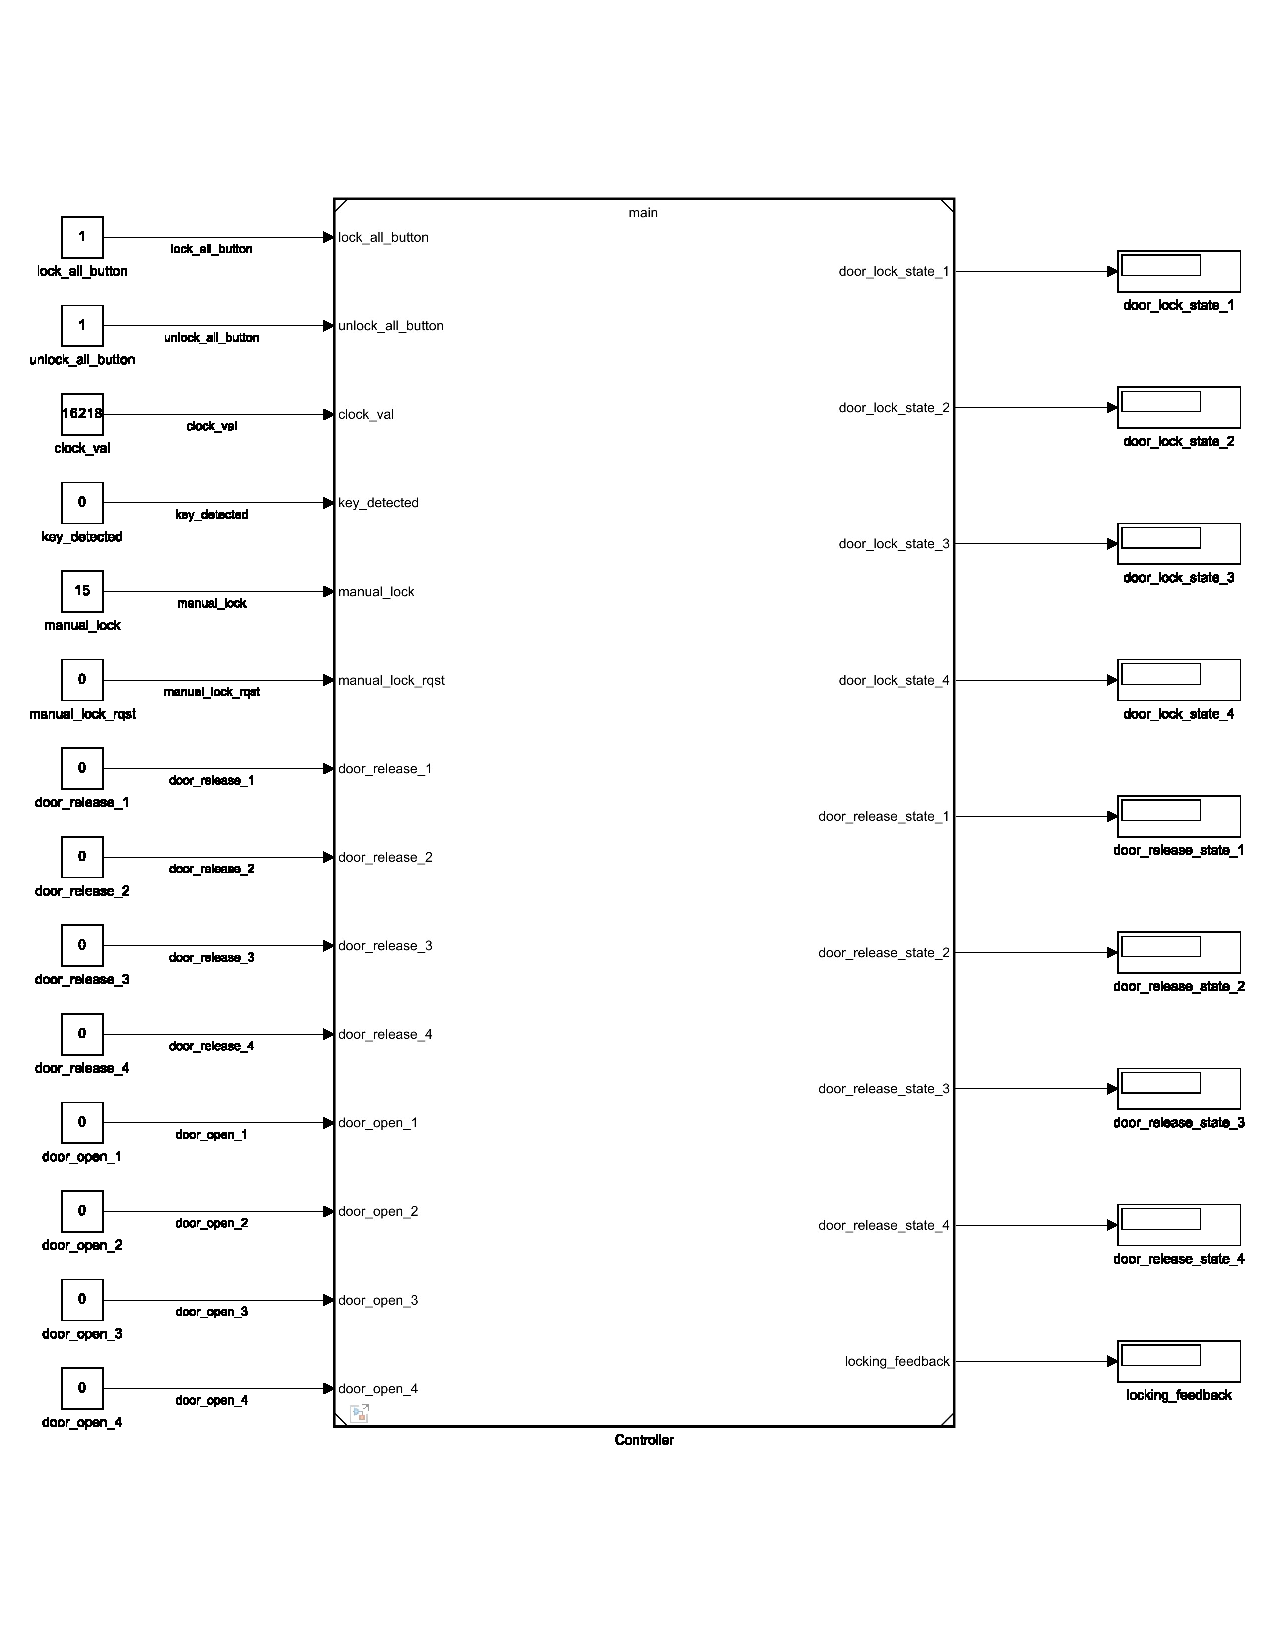
\includepdf[pages=-]{anexos/feature_model.pdf}

\end{anexosenv}


\end{document}
